\documentclass[9pt,dvipsnames,table,UTF8,aspectratio=169]{beamer}
\usepackage[no-math,cm-default]{fontspec}
\usepackage[indentfirst]{xeCJK}
\usepackage{amsmath}
\usepackage{amsthm}
\usepackage{amssymb}
\usepackage{ctex}
\usepackage{comment}
\usepackage{verbatim}
\usepackage{indentfirst}
\usepackage{syntonly}
% 图像支持
\usepackage{graphicx}
\usepackage{paralist}
\usepackage{beamerthemesplit}
\usepackage{ulem}
\usepackage{listings}
\usepackage{etoolbox}
\usepackage{endnotes}
\usepackage{zhspacing}

% Font
\usefonttheme{professionalfonts}
\setCJKmainfont[BoldFont={SimHei},ItalicFont={KaiTi}]{SimSun}
\setCJKsansfont{SimSun}
\setmonofont[Scale=0.8]{Monaco}
\CJKsetecglue{}
\setbeamerfont{section in toc}{size=\fontsize{10pt}{\baselineskip}}

% Theme
\usetheme{Antibes}
\usecolortheme{beaver}

\newcommand{\hlink}[1]{
	\footnote{\fontsize{6pt}{\baselineskip}\href{#1}{\textsl{\underline{#1}}}}
}
\newcommand{\graph}[2]
{\begin{figure}[h]
	\centering
	\includegraphics[width=#2 \textwidth]{image/#1}
\end{figure}}

\lstset{language=C++,
	extendedchars=false,
	basicstyle=\ttfamily\footnotesize,
	keywordstyle=\bfseries\color{blue},
	identifierstyle=\color{blue!60!black},
	commentstyle=\itshape\color{gray},
	escapeinside=`'}


\setlength{\parindent}{2em}
\setlength{\baselineskip}{1.3\baselineskip}

\setbeamercolor{math text}{fg=black}
\setbeamertemplate{qed symbol}{ $ \square $ }
\setbeamerfont{headline}{size=\fontsize{6.5pt}{\baselineskip}}
\setbeamerfont{footline}{size=\fontsize{6.5pt}{\baselineskip}}
\setbeamertemplate{theorems}[numbered]
\renewcommand{\thetheorem}{\arabic{subsubsection}.\arabic{theorem}}
\renewcommand{\thelemma}{\arabic{subsubsection}.\arabic{lemma}}
\newenvironment{qedf}{%
	\begin{frame}[environment=qedqedframe]%
	}{%
	\qed
	\end{frame}%
}
\renewcommand{\appendixname}{结语}

\makeatletter
\patchcmd{\beamer@sectionintoc}{\vskip 1.5em}{\vskip 1em}{}{}
\makeatother

\begin{document}
\AtBeginSection[] 
{
	\begin{frame}
		\tableofcontents[currentsection, hideallsubsections]
	\end{frame}
}

\AtBeginSubsection[]
{
	\begin{frame}[shrink]
		\tableofcontents[sectionstyle=show/shaded, subsectionstyle=show/shaded/hide]
	\end{frame}
}

% document info
\title{最大团作业~~实验报告}
\subtitle{Maximum Clique}
\author{周尚彦}
\institute{北京大学~~信息科学技术学院}
\date{May. 30$^{\text{th}}$}

\maketitle

\begin{frame}
	\frametitle{Contents}
	
	\tableofcontents[hideallsubsections]
\end{frame}

\section{简介}
\subsection{基本概念}
\begin{frame}{定义}
\begin{definition}{团}
	给定一个无向图$G = (V,E)$,团(Clique)是指图$G$顶点集的一个子集$C \subseteq V$,其中的任意两顶点都邻接。
\end{definition}

\begin{definition}{团问题}
	给定一个无向图$G = (V, E)$和常数$k$,团问题要求确定图中是否包含一个规模为$k$的团。
\end{definition}

\begin{definition}{最大团问题}
	给定一个无向图$G = (V, E)$,最大团(Maximum Clique)问题要求找出一个具有最大规模的团。
\end{definition}
\end{frame}

\begin{frame}{NP完全性}
	\begin{itemize}
		\item 3-CNF-SAT问题可以在多项式时间内归约到团问题
		\item 3-CNF-SAT问题是NP完全的
		\item 最大团问题和团问题是等价的
	\end{itemize}

	所以最大团问题是NP完全的。
\end{frame}

\begin{frame}{最小顶点覆盖问题}
	\begin{definition}{顶点覆盖}
		给定一个无向图$G = (V,E)$,顶点覆盖(Vertex Cover)是指图$G$顶点集的一个子集$C \subseteq V$,使得$G$的每一条边都有一个点属于$C$。
	\end{definition}

	\begin{definition}{最小顶点覆盖问题}
		给定一个无向图$G = (V,E)$,最小顶点覆盖(Minimum Vertex Cover)问题要求找出一个具有最小规模的顶点覆盖。
	\end{definition}

	一个顶点集合$K$是$G$的一个团当且仅当$V \backslash K$是补图$G$的一个顶点覆盖。
\end{frame}

\begin{frame}{最大独立集}
	\begin{definition}{独立集}
		给定一个无向图$G = (V,E)$,独立集(Independent Set)是指图$G$顶点集的一个子集$C \subseteq V$,其中的任意两顶点都不邻接。
	\end{definition}

	\begin{definition}{最小顶点覆盖问题}
		给定一个无向图$G = (V,E)$,最大独立集(Maximum Independent Set)问题要求找出一个具有最大基数的独立集。
	\end{definition}

	一个顶点集合$S$是$G$的一个独立集当且仅当$V \backslash S$是$G$的一个顶点覆盖。
\end{frame}

\subsection{问题研究历史及现状简述}
\begin{frame}{确定性算法}
	Hararv首先提出最大团问题的确定性算法\footnotemark。

	最早的解决最大团问题的精确算法是枚举法(enumerative algorithms)。

	目前常用的确定性算法有分支限界法(Brandand  bound)\footnotemark 和回溯法(Backtracking  Algorithm)等。

	\footnotetext[1]{HARARV F. Combinatorial problems on graphical enumeration, Chapter 6 in EF Bechenbach (Ed.): Applied Combinatorial Mathematics[J]. 1964. }
	\footnotetext[2]{Tomita E, Sutani Y, Higashi T, et al. A simple and faster branch-and-bound algorithm for finding a maximum clique[M]//WALCOM: Algorithms and computation. Springer Berlin Heidelberg, 2010: 191-203.}
\end{frame}

\begin{frame}{启发式算法}
	相比于确定性算法,启发式方法求解最大团问题并不能得到图的精确的最大团,只能在规定的计算范围内得到最好的团。但启发式算法更适用于规模较大的问题。

	目前常用的启发式算法有RLS(Reactive Local search)\footnotemark、DAGS(Deep Adaptive Greedy Search)\footnotemark、GLS(Genetic Local Search )\footnotemark。

	其他启发式算法还有带有贪婪随机自适应搜索过程(GRASP)的算法、人工神经网络(ANN)、禁忌搜索(TS)、可变近邻搜索(VNS)、模拟退火算法,遗传算法等。 

	\footnotetext[3]{Battiti  R,  Protasi  M.  Reactive  local  search  for  the  maximum  clique  problem  1[J].  Algorithmica, 2001, 29(4): 610-637. }
	\footnotetext[4]{Grosso A, Locatelli M, Della Croce F. Combining swaps and node weights in an adaptive greedy approach for the maximum clique problem[J]. Journal of Heuristics, 2004, 10(2): 135-152. }
	\footnotetext[5]{Marchiori  E.  Genetic,  iterated  and  multistart  local  search  for  the  maximum  clique problem[M]//Applications of Evolutionary Computing. Springer Berlin Heidelberg, 2002: 112-121. }
\end{frame}

\section{边加权局部搜索(Edge Weight Local Search)}
\subsection{基本概念}
\begin{frame}{局部搜索}
	局部搜索(Local Search)是一种最求解优化问题的方法。
	
	定义好候选解的领域结构之后,问题的解空间就可以看成一个图。
	
	局部搜索算法从解空间的一个点出发,每一步从当前候选解移动到一个邻居候选解,去寻找较好的候选解,候选解的质量是由一个评估函数来界定的。

	局部搜索算法从当前候选解跳转到邻居解的时候,只根据有限的局部信息来做决定。
\end{frame}

\begin{frame}
	简单局部搜索算法主要有:迭代改进,随机游动,随机迭代改进,简单禁忌搜索等。
	\begin{itemize}
		\item 迭代改进(Iterative Improvement):也称为爬山法,每次从当前候选解的邻居候选解中选择一个最优解进行转移,直到达到一个局部最优解。
		\item 随机游动(Random Walk):每次从当前候选解的邻居中随机地选取一个进行转移。
		\item 随机迭代改进(Random Iterative Improvement):每个搜索步首先产生一个随机数$r \in [0, 1]$,然后以$r$的概率进行随机游动,以$1 - r$的概率进行迭代改进。
		\item 简单禁忌搜索(Simple Tabu Search)每个搜索步都从没被禁忌的邻居中选择一个最优的候选解进行转移。
	\end{itemize}
\end{frame}

\begin{frame}{评估函数}
	EWLS用于直接求解最小顶点覆盖问题。

	在EWLS中,给定的无向图被转换成一个边加权无向图。由原来的无向图$G = (V,E)$结合一个加权函数$w$构成,使得$\forall e \in E$都有一个正整数$w(e)$作为它的权值。

	其中$w(e)$的初值为$1$,且会随着算法的进行发生改变。

	一个候选解$X$的代价由公式$$cost(G,X) = \sum_{e isn't covered by X} w(e)$$给出。

	改变顶点$v \in V$的选择状态对当前候选解代价的贡献记为$dscore(v)$。
\end{frame}

\begin{frame}{部分顶点覆盖}
	\begin{definition}{部分顶点覆盖}
		对于一个无向图$G = (V,E)$, 我们说一个大小为$k$的顶点子集$P \subseteq V$是一个$(k, t)-$部分顶点覆盖(partial vertex cover),简称$(k, t)-PVC (0 \le t \le |E|)$,如果$P$覆盖了$G$的$|E| − t$条边。
	\end{definition}

	\begin{theorem}
		对于一个无向图$G = (V,E)$,$G$的一个$(k, t)-PVC$对该图的最小顶点覆盖的规模提供了一个$k + t$的上界。
	\end{theorem}

	EWLS算法的思想就是找到一个比较优化的部分顶点覆盖,然后把它扩展为一个完整的顶点覆盖。
\end{frame}

\subsection{算法流程}
\begin{frame}{预备工作}
	\begin{itemize}
		\item 初始化所有的边权和$dscore$
		\item 贪心选择$dscore$最大的点,求一个解初始解$C$,并将其赋值为当前最优解$C'$。
		\item 由$C$和给定参数$delta$贪心地选择$dscore$最大的点从当前解中除去,得到一个规模为$|C| - delta$的候选解。
	\end{itemize}
\end{frame}

\begin{frame}{搜索步骤}
	\begin{itemize}
		\item 根据每条未被选择的边的持续未被选择时间和每个点的$dscore$抽取出已在当前候选解中的点$u$和未在当前候选解中的点$v$。
		\item 在抽取点的同时检查候选解是否陷入局部最优,视情况更新边权。
		\item 置换$(u,v)$的被选择状态,获得新的候选解。
		\item 使用候选解更新答案。
	\end{itemize}
\end{frame}

\section{实验结果}
\subsection{实验环境}
\begin{frame}{实验平台}
	\begin{columns}
		\begin{column}{0.5\textwidth}
			实验平台1:
			
			CPU:Intel® Core™ i5-6200U Processor

			RAM:4G + 8G Dual Channel

			System:Windows 10 Professional x64
		\end{column}
		\begin{column}{0.5\textwidth}
			实验平台2:

			CPU:Intel® Core™ i7-6700HQ Processor

			RAM:8G

			System:Windows 10 Home Edition x64
		\end{column}
	\end{columns}
\end{frame}

\begin{frame}{实验代码及数据}
	EWLS算法使用C++语言实现,编译器为mingw-w64 7.1.0,编译过程中开启了O3优化。

	测试代码和统计数据代码使用Python3.6.1实现,使用time.time()函数计算代码运行时间\footnotemark。

	采用来自\url{http://www.nlsde.buaa.edu.cn/~kexu/benchmarks/graph-benchmarks.htm}的测试数据。

	\footnotetext[6]{实验结果中的平均用时和中位用时均只考虑跑出最优解的测试组。}
\end{frame}

\begin{frame}{实验停止标准}
	在输入参数给定了输入数据对应的最优解的值,当程序运行至求得最优解时,程序会自动退出。

	由于最小顶点覆盖问题的难解性,对于大规模的输入数据,程序常常无法求得最优解。

	设置$maxSteps = 5000000$,当搜索进行$maxSteps$步时,程序会自动退出并输出当前找到的最优解。
\end{frame}

\subsection{结果展示}
\begin{frame}
	\begin{figure}[H]
		\centering
		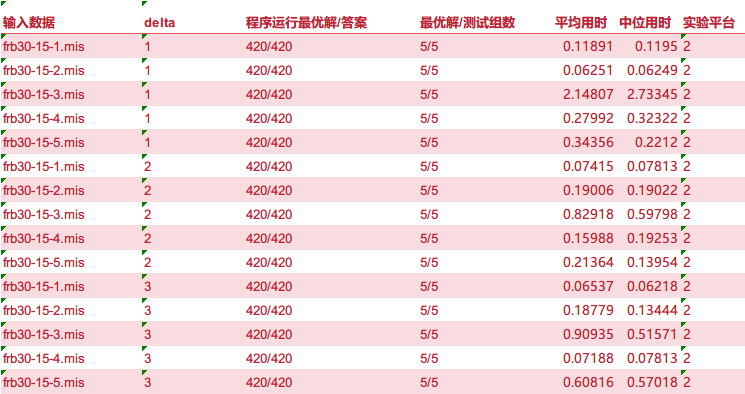
\includegraphics[width=0.8\textwidth]{0.png}
		\caption{实验结果-0}\label{results}
	\end{figure}
\end{frame}

\begin{frame}
	\begin{figure}[H]
		\centering
		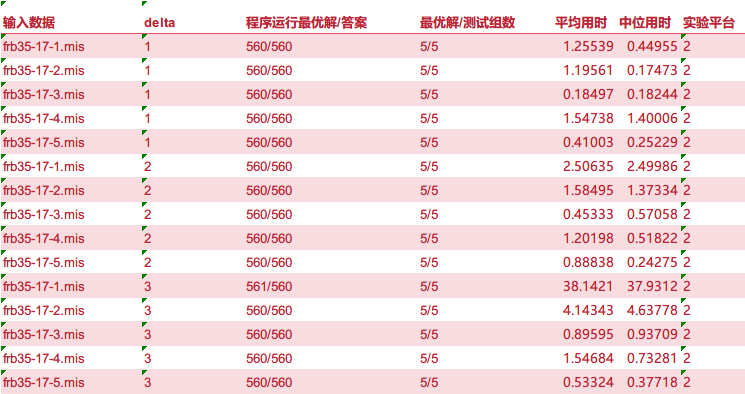
\includegraphics[width=0.8\textwidth]{1.png}
		\caption{实验结果-1}\label{results}
	\end{figure}
\end{frame}

\begin{frame}
	\begin{figure}[H]
		\centering
		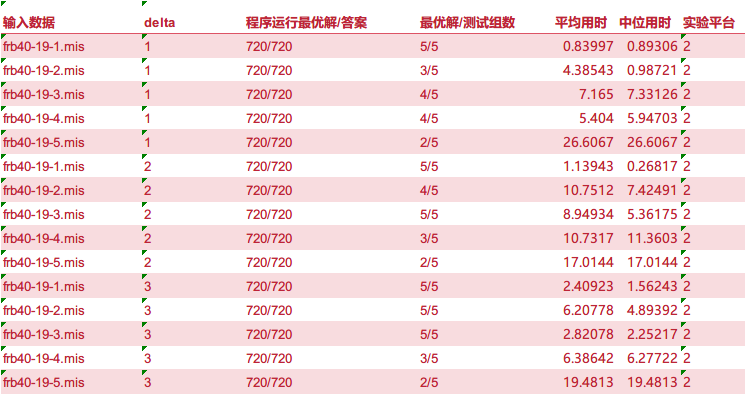
\includegraphics[width=0.8\textwidth]{2.png}
		\caption{实验结果-2}\label{results}
	\end{figure}
\end{frame}

\begin{frame}
	\begin{figure}[H]
		\centering
		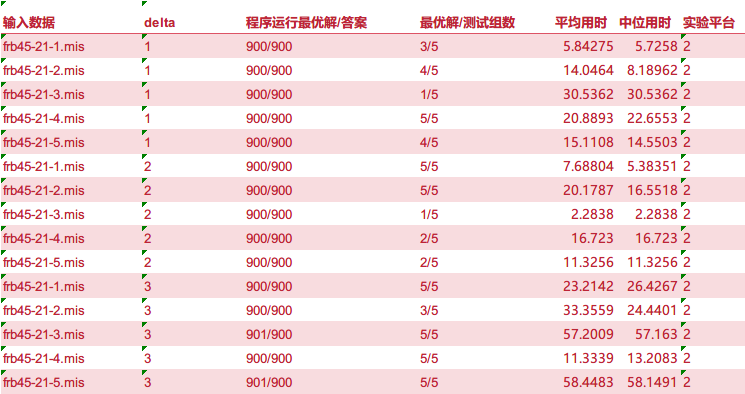
\includegraphics[width=0.8\textwidth]{3.png}
		\caption{实验结果-3}\label{results}
	\end{figure}
\end{frame}

\begin{frame}
	\begin{figure}[H]
		\centering
		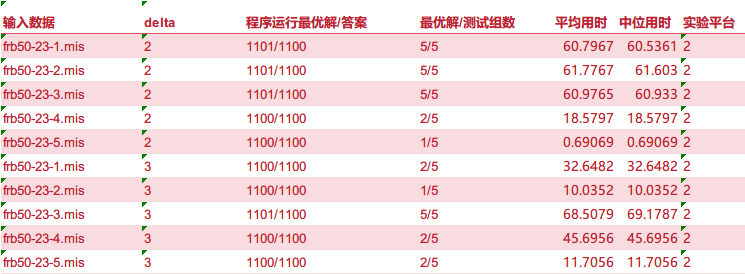
\includegraphics[width=0.8\textwidth]{4.png}
		\caption{实验结果-4}\label{results}
	\end{figure}
\end{frame}

\begin{frame}
	\begin{figure}[H]
		\centering
		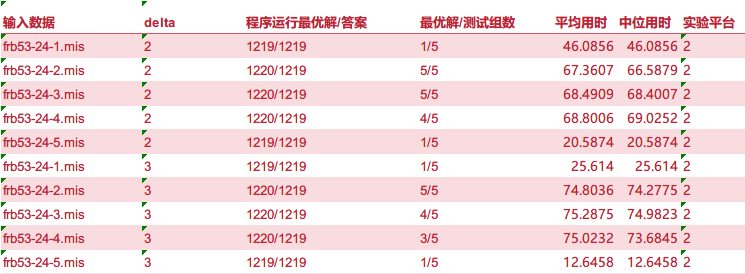
\includegraphics[width=0.8\textwidth]{5.png}
		\caption{实验结果-5}\label{results}
	\end{figure}
\end{frame}

\begin{frame}
	\begin{figure}[H]
		\centering
		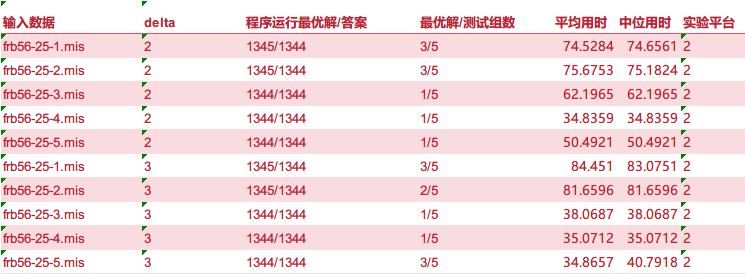
\includegraphics[width=0.8\textwidth]{6.png}
		\caption{实验结果-6}\label{results}
	\end{figure}
\end{frame}

\begin{frame}
	\begin{figure}[H]
		\centering
		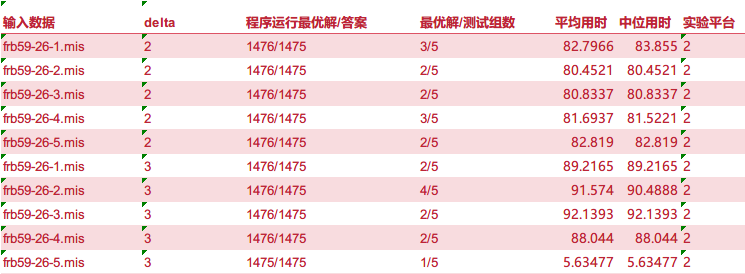
\includegraphics[width=0.8\textwidth]{7.png}
		\caption{实验结果-7}\label{results}
	\end{figure}
\end{frame}

\begin{frame}
	\begin{figure}[H]
		\centering
		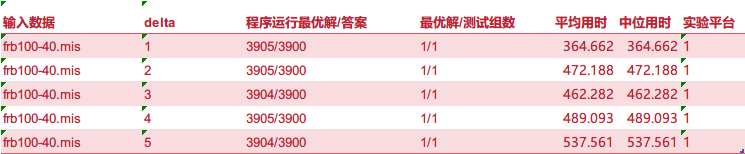
\includegraphics[width=0.8\textwidth]{8.png}
		\caption{实验结果-8}\label{results}
	\end{figure}
\end{frame}

\appendix
\section{}
\begin{frame}{Fin.}
	The end.

	Thanks.
\end{frame}

\end{document}
